\documentclass[a4papper, 10pt]{article}

 \usepackage[utf8]{inputenc}
 \usepackage[T1]{fontenc}
 \usepackage[normalem]{ulem}
 \usepackage[british]{babel}
 \usepackage{graphicx}
 \usepackage{caption}
 \usepackage{subcaption}
 \usepackage{enumerate}
 \usepackage{array}
 \usepackage{amsmath,amssymb,mathrsfs}
 \usepackage{url}
 \usepackage{fullpage}
 \usepackage[table]{xcolor}
 \usepackage{placeins} 
 
 \definecolor{light-gray}{gray}{0.85}
 %\newcolumntype{M}[1]{>{\raggedright}m{#1}}
 \newcolumntype{M}[1]{>{\centering\arraybackslash}m{#1}} % To center text in table

 \title{Report: CS02 electrical validation}
 \author{Benjamin Boitrelle}
 \date{November 2015}

 \begin{document}

    \maketitle
    \tableofcontents

  %\section{Alignment and bounding inspection}
  \section{Electrical tests}
    \subsection{Auxiliary board}
    
   Here, some parameters of the auxiliary board are measured.
   \begin{itemize}
     \item Consumption: 378 mA
     \item $V_{clp} \ = \ 2.1 \ V$
     \item $V_{dd_D} \ = \ 3.357 \ V$
     \item $V_{dd_A} \ = \ 3.301 \ V$
   \end{itemize}

     \subsection{CS02 smoke test}

    First smoke test done without changing the value of  $V_{clp}$, $V_{dd_D}$ of $V_{dd_A}$:
     \begin{itemize}
       \item POWER ON: 33 mA
       \item RESET: 33 mA
       \item ALL: 750 mA
       \item READ: 750 mA and no error sent by the JTAG software
       \item START: 1128 mA
     \end{itemize}

     Measurement of voltages at the capacitors close to the connector:
     
     \begin{itemize}
       \item $V_{clp} \ = \ 2.072 \ V$ adjusted to 2.108 V
       \item $V_{dd_D} \ = \ 2.923 \ V$ adjusted to 3.337 V
       \item $V_{dd_A} \ = \ 2.746 \ V$ adjusted to 3.345 V
     \end{itemize}

     Second smoke test done after recalibrating $V_{clp}$, $V_{dd_D}$ of $V_{dd_A}$:
     
     \begin{itemize}
       \item POWER ON: 1461 mA
       \item RESET: 40 mA
       \item ALL: 829 mA
       \item READ: 829 mA and no error sent by the JTAG software
       \item START: 1402 mA
     \end{itemize}
 
  \section{Calibration}
    \subsection{Sensors output checked on the oscilloscope}

     \begin{itemize}
       \item[Chip 1:]
         \begin{itemize}
            \item RESET/JTAG: OK
            \item Control Header/Trailer: OK
            \item No dead pixel
         \end{itemize}  
       \item[Chip 2:]
         \begin{itemize}
            \item RESET/JTAG: OK
            \item Control Header/Trailer: OK
            \item No dead pixel
         \end{itemize}  
       \item[Chip 3:]
         \begin{itemize}
            \item RESET/JTAG: OK
            \item Control Header/Trailer: OK
            \item Dead pixels
         \end{itemize}  
       \item[Chip 4:]
         \begin{itemize}
            \item RESET/JTAG: OK
            \item Control Header/Trailer: OK
            \item No dead pixel
         \end{itemize}  
       \item[Chip 5:]
         \begin{itemize}
            \item RESET/JTAG: OK
            \item Control Header/Trailer: OK
            \item No dead pixel
         \end{itemize}  
       \item[Chip 6:]
         \begin{itemize}
            \item RESET/JTAG: OK
            \item Control Header/Trailer: OK
            \item No dead pixel
         \end{itemize}  
     \end{itemize}

    \subsection{DAQ calibration}

      \subsubsection{Chip 1}

      Few pixels are stuck to 1 on the sub-matrix C.

      \begin{itemize}

          \item Estimation of the "middle points":
          \begin{center}
            \begin{tabular}{|c|c|c|c|c|}
              \hline %-------------------------------------------------------------------------------------
             \rowcolor{light-gray} $V_{ref_2}$  &   $V_{ref_{1A}}$  &   $V_{ref_{1B}}$  &   $V_{ref_{1C}}$  &   $V_{ref_{1D}}$  \tabularnewline
              \hline %-------------------------------------------------------------------------------------
              100        &        112        &         115       &       179         &        155        \tabularnewline
              \hline %-------------------------------------------------------------------------------------
            \end{tabular}
          \end{center}

          \item Discriminators calibration:
          \begin{center}
            \begin{tabular}{|M{1.3cm}|M{1.3cm}|M{1.3cm}|M{1.3cm}|M{1.3cm}|M{1.3cm}|M{1.3cm}|M{1.3cm}|M{1.3cm}|}
              \hline %-------------------------------------------------------------------
             \rowcolor{light-gray} $V_{ref1_A}$ START  & $V_{ref1_B}$ START & $V_{ref1_C}$ START & $V_{ref1_D}$ START & $V_{ref2}$ & $V_{ref1_A}$ STOP & Step & Event nb / step & Number of Runs \tabularnewline
              \hline %-------------------------------------------------------------------
                84  &  87  &  151  & 127  &  100  &  140  &  2  &  500  &  29  \tabularnewline
              \hline %-------------------------------------------------------------------
            \end{tabular}
          \end{center}

          \item Temporal noise, fixed pattern noise and offset:

            \begin{center}
              \begin{tabular}{|c|c|c|c|}
                \hline %----------------------------
         \rowcolor{light-gray}         Matrix  &  TN   &  FPN  &  Offset  \tabularnewline
                \hline %----------------------------
                    A     & 1.072 & 0.313 & 0.253    \tabularnewline
                \hline %----------------------------
                    B     & 1,287 & -0.611 & 0,968   \tabularnewline
                \hline %----------------------------
                    C     & 0.948 & 0.388 & 0.911   \tabularnewline
                \hline %----------------------------
                    D     & 0.936 & 0.362 & 0.644    \tabularnewline
                \hline %----------------------------
              \end{tabular}
            \end{center}
        
        \item Fake Hit Rate estimation (DAQ values = middle point values + 20 and accumulation of $10^4$ events): 2.9 hits/frame
         
        \item \textbf{Observations:} Few pixels are stuck to 0 on the sub-matrix C (col 731 line 48 to 64).
        
        \end{itemize}

             \subsubsection{Chip 2}

      \begin{itemize}

          \item Estimation of the "middle points":
          \begin{center}
            \begin{tabular}{|c|c|c|c|c|}
              \hline %-------------------------------------------------------------------------------------
             \rowcolor{light-gray} $V_{ref_2}$  &   $V_{ref_{1A}}$  &   $V_{ref_{1B}}$  &   $V_{ref_{1C}}$  &   $V_{ref_{1D}}$  \tabularnewline
              \hline %-------------------------------------------------------------------------------------
              100        &        139       &         127       &       158         &        115        \tabularnewline
              \hline %-------------------------------------------------------------------------------------
            \end{tabular}
          \end{center}

          \item Discriminators calibration:
          \begin{center}
            \begin{tabular}{|M{1.3cm}|M{1.3cm}|M{1.3cm}|M{1.3cm}|M{1.3cm}|M{1.3cm}|M{1.3cm}|M{1.3cm}|M{1.3cm}|}
              \hline %-------------------------------------------------------------------
             \rowcolor{light-gray} $V_{ref1_A}$ START  & $V_{ref1_B}$ START & $V_{ref1_C}$ START & $V_{ref1_D}$ START & $V_{ref2}$ & $V_{ref1_A}$ STOP & Step & Event nb / step & Number of Runs \tabularnewline
              \hline %-------------------------------------------------------------------
                111  &  99  &  130  & 87  &  100  &  167  &  2  &  500  &  29  \tabularnewline
              \hline %-------------------------------------------------------------------
            \end{tabular}
          \end{center}

          \item Temporal noise, fixed pattern noise and offset:

            \begin{center}
              \begin{tabular}{|c|c|c|c|}
                \hline %----------------------------
         \rowcolor{light-gray}         Matrix  &  TN   &  FPN  &  Offset  \tabularnewline
                \hline %----------------------------
                    A     & 1.143 & 0.386 & 0.257    \tabularnewline
                \hline %----------------------------
                    B     & 1.188 & -0.175 & 0.955   \tabularnewline
                \hline %----------------------------
                    C     & 1.104 & -0.358 & 1.074   \tabularnewline
                \hline %----------------------------
                    D     & 1.028 & 0.652 & 0.573    \tabularnewline
                \hline %----------------------------
              \end{tabular}
            \end{center}

        \item Fake Hit Rate estimation (DAQ values = middle point values + 20 and accumulation of $10^4$ events): 16.4 hits/frame
         
       \end{itemize}

      \subsubsection{Chip 3}

      \begin{itemize}

          \item Estimation of the "middle points":
          \begin{center}
            \begin{tabular}{|c|c|c|c|c|}
              \hline %-------------------------------------------------------------------------------------
             \rowcolor{light-gray} $V_{ref_2}$  &   $V_{ref_{1A}}$  &   $V_{ref_{1B}}$  &   $V_{ref_{1C}}$  &   $V_{ref_{1D}}$  \tabularnewline
              \hline %-------------------------------------------------------------------------------------
              100        &        148       &         140       &       153         &        126        \tabularnewline
              \hline %-------------------------------------------------------------------------------------
            \end{tabular}
          \end{center}

          \item Discriminators calibration:
          \begin{center}
            \begin{tabular}{|M{1.3cm}|M{1.3cm}|M{1.3cm}|M{1.3cm}|M{1.3cm}|M{1.3cm}|M{1.3cm}|M{1.3cm}|M{1.3cm}|}
              \hline %-------------------------------------------------------------------
             \rowcolor{light-gray} $V_{ref1_A}$ START  & $V_{ref1_B}$ START & $V_{ref1_C}$ START & $V_{ref1_D}$ START & $V_{ref2}$ & $V_{ref1_A}$ STOP & Step & Event nb / step & Number of Runs \tabularnewline
              \hline %-------------------------------------------------------------------
              120  & 112  &  130  & 98  &  100  &  176  &  2  &  500  &  29  \tabularnewline
              \hline %-------------------------------------------------------------------
            \end{tabular}
          \end{center}

          \item Temporal noise, fixed pattern noise and offset:

            \begin{center}
              \begin{tabular}{|c|c|c|c|}
                \hline %----------------------------
         \rowcolor{light-gray}         Matrix  &  TN   &  FPN  &  Offset  \tabularnewline
                \hline %----------------------------
                    A     & 1.087 & 0.445 & 0.240    \tabularnewline
                \hline %----------------------------
                    B     & 1.094 &  0.129 & 0.832   \tabularnewline
                \hline %----------------------------
                    C     & 1.013 & -0.377 & 0.962   \tabularnewline
                \hline %----------------------------
                    D     & 0.947 & 1.022 & 0.356    \tabularnewline
                \hline %----------------------------
              \end{tabular}
            \end{center}

        \item Fake Hit Rate estimation (DAQ values = middle point values + 20 and accumulation of $10^4$ events): 367 hits/frame
        
        \item \textbf{Observations:} One column on sub-matrix D stuck to 0 (col: 1145). Strange pattern seen on the test monitoring to estimate the fake hit rate (see picture).
        
        \end{itemize}

      \subsubsection{Chip 4}

      \begin{itemize}

          \item Estimation of the "middle points":
          \begin{center}
            \begin{tabular}{|c|c|c|c|c|}
              \hline %-------------------------------------------------------------------------------------
             \rowcolor{light-gray} $V_{ref_2}$  &   $V_{ref_{1A}}$  &   $V_{ref_{1B}}$  &   $V_{ref_{1C}}$  &   $V_{ref_{1D}}$  \tabularnewline
              \hline %-------------------------------------------------------------------------------------
              100        &         95       &         146       &       161         &        169        \tabularnewline
              \hline %-------------------------------------------------------------------------------------
            \end{tabular}
          \end{center}

          \item Discriminators calibration:
          \begin{center}
            \begin{tabular}{|M{1.3cm}|M{1.3cm}|M{1.3cm}|M{1.3cm}|M{1.3cm}|M{1.3cm}|M{1.3cm}|M{1.3cm}|M{1.3cm}|}
              \hline %-------------------------------------------------------------------
             \rowcolor{light-gray} $V_{ref1_A}$ START  & $V_{ref1_B}$ START & $V_{ref1_C}$ START & $V_{ref1_D}$ START & $V_{ref2}$ & $V_{ref1_A}$ STOP & Step & Event nb / step & Number of Runs \tabularnewline
              \hline %-------------------------------------------------------------------
               67  & 118  &  133  & 141 &  100  &  176  &  2  &  500  &  29  \tabularnewline
              \hline %-------------------------------------------------------------------
            \end{tabular}
          \end{center}

          \item Temporal noise, fixed pattern noise and offset:

            \begin{center}
              \begin{tabular}{|c|c|c|c|}
                \hline %----------------------------
         \rowcolor{light-gray}         Matrix  &  TN   &  FPN  &  Offset  \tabularnewline
                \hline %----------------------------
                    A     & 1.081 & 0.340 & 0.321    \tabularnewline
                \hline %----------------------------
                    B     & 1.228 & -0.244 & 0.880   \tabularnewline
                \hline %----------------------------
                    C     & 0.956 & -0.089 & 1.003   \tabularnewline
                \hline %----------------------------
                    D     & 0.929 & 0.702 & 0.387    \tabularnewline
                \hline %----------------------------
              \end{tabular}
            \end{center}

        \item Fake Hit Rate estimation (DAQ values = middle point values + 20 and accumulation of $10^4$ events): 14.7 hits/frame
        
        %\item \textbf{Observations:} One column on sub-matrix D stuck to 0 (col: 1145). Strange pattern seen on the test monitoring to estimate the fake hit rate (see picture).
        
        
        \end{itemize}

        \subsubsection{Chip 5}

      \begin{itemize}

          \item Estimation of the "middle points":
          \begin{center}
            \begin{tabular}{|c|c|c|c|c|}
              \hline %-------------------------------------------------------------------------------------
             \rowcolor{light-gray} $V_{ref_2}$  &   $V_{ref_{1A}}$  &   $V_{ref_{1B}}$  &   $V_{ref_{1C}}$  &   $V_{ref_{1D}}$  \tabularnewline
              \hline %-------------------------------------------------------------------------------------
              100        &         86       &         125       &       173         &        185        \tabularnewline
              \hline %-------------------------------------------------------------------------------------
            \end{tabular}
          \end{center}

          \item Discriminators calibration:
          \begin{center}
            \begin{tabular}{|M{1.3cm}|M{1.3cm}|M{1.3cm}|M{1.3cm}|M{1.3cm}|M{1.3cm}|M{1.3cm}|M{1.3cm}|M{1.3cm}|}
              \hline %-------------------------------------------------------------------
             \rowcolor{light-gray} $V_{ref1_A}$ START  & $V_{ref1_B}$ START & $V_{ref1_C}$ START & $V_{ref1_D}$ START & $V_{ref2}$ & $V_{ref1_A}$ STOP & Step & Event nb / step & Number of Runs \tabularnewline
              \hline %-------------------------------------------------------------------
               58  &  97  &  145  & 157 &  100  &  114  &  2  &  500  &  29  \tabularnewline
              \hline %-------------------------------------------------------------------
            \end{tabular}
          \end{center}

          \item Temporal noise, fixed pattern noise and offset:

            \begin{center}
              \begin{tabular}{|c|c|c|c|}
                \hline %----------------------------
         \rowcolor{light-gray}         Matrix  &  TN   &  FPN  &  Offset  \tabularnewline
                \hline %----------------------------
                    A     & 1.031 & 0.254 & 0.323    \tabularnewline
                \hline %----------------------------
                    B     & 0.993 &  0.134 & 0.715   \tabularnewline
                \hline %----------------------------
                    C     & 0.864 &  0.450 & 0.874   \tabularnewline
                \hline %----------------------------
                    D     & 0.903 & 0.284 & 0.461    \tabularnewline
                \hline %----------------------------
              \end{tabular}
            \end{center}

        \item Fake Hit Rate estimation (DAQ values = middle point values + 20 and accumulation of $10^4$ events): 3.3 hits/frame (sub-matrix C Vref value a bit too low)
        
        %\item \textbf{Observations:} One column on sub-matrix D stuck to 0 (col: 1145). Strange pattern seen on the test monitoring to estimate the fake hit rate (see picture).
               
        \end{itemize}

        \subsubsection{Chip 6}

      \begin{itemize}

          \item Estimation of the "middle points":
          \begin{center}
            \begin{tabular}{|c|c|c|c|c|}
              \hline %-------------------------------------------------------------------------------------
             \rowcolor{light-gray} $V_{ref_2}$  &   $V_{ref_{1A}}$  &   $V_{ref_{1B}}$  &   $V_{ref_{1C}}$  &   $V_{ref_{1D}}$  \tabularnewline
              \hline %-------------------------------------------------------------------------------------
              100        &        171       &         162       &       189         &        151        \tabularnewline
              \hline %-------------------------------------------------------------------------------------
            \end{tabular}
          \end{center}

          \item Discriminators calibration:
          \begin{center}
            \begin{tabular}{|M{1.3cm}|M{1.3cm}|M{1.3cm}|M{1.3cm}|M{1.3cm}|M{1.3cm}|M{1.3cm}|M{1.3cm}|M{1.3cm}|}
              \hline %-------------------------------------------------------------------
             \rowcolor{light-gray} $V_{ref1_A}$ START  & $V_{ref1_B}$ START & $V_{ref1_C}$ START & $V_{ref1_D}$ START & $V_{ref2}$ & $V_{ref1_A}$ STOP & Step & Event nb / step & Number of Runs \tabularnewline
              \hline %-------------------------------------------------------------------
               143 &  134 &  161  & 123 &  100  &  199  &  2  &  500  &  29  \tabularnewline
              \hline %-------------------------------------------------------------------
            \end{tabular}
          \end{center}

          \item Temporal noise, fixed pattern noise and offset:

            \begin{center}
              \begin{tabular}{|c|c|c|c|}
                \hline %----------------------------
         \rowcolor{light-gray}         Matrix  &  TN   &  FPN  &  Offset  \tabularnewline
                \hline %----------------------------
                    A     & 0.985 & 0.447 & 0.297    \tabularnewline
                \hline %----------------------------
                    B     & 1.076 & -0.032 & 0.768   \tabularnewline
                \hline %----------------------------
                    C     & 1.019 & -0.613 & 0.977   \tabularnewline
                \hline %----------------------------
                    D     & 0.846 & 0.838 & 0.389    \tabularnewline
                \hline %----------------------------
              \end{tabular}
            \end{center}

        \item Fake Hit Rate estimation (DAQ values = middle point values + 20 and accumulation of $10^4$ events): 0.6 hits/frame (sub-matrix C Vref value a bit too low)
        
        %\item \textbf{Observations:} One column on sub-matrix D stuck to 0 (col: 1145). Strange pattern seen on the test monitoring to estimate the fake hit rate (see picture).
               
        \end{itemize}

  The fake hit rate measurements was done in the test beam acquisition mode. The acquisition was done in the dark, for different thresholds and $5.10^6$ events were recorded per run.

  \begin{center}
    \begin{tabular}{|c|c|c|}
      \hline %----------------------------
   \rowcolor{light-gray}  Sensors  &  Run number  &  Thresholds  ($\sigma$) \tabularnewline
      \hline %----------------------------
      1-2   &   7078   &    3 \tabularnewline
      \hline %----------------------------
      1-2   &   7079   &    5 \tabularnewline
      \hline %----------------------------
      1-2   &   7080   &    7 \tabularnewline
      \hline %----------------------------
    \end{tabular}
  \end{center}
        \begin{figure}[!h]
            \centering
            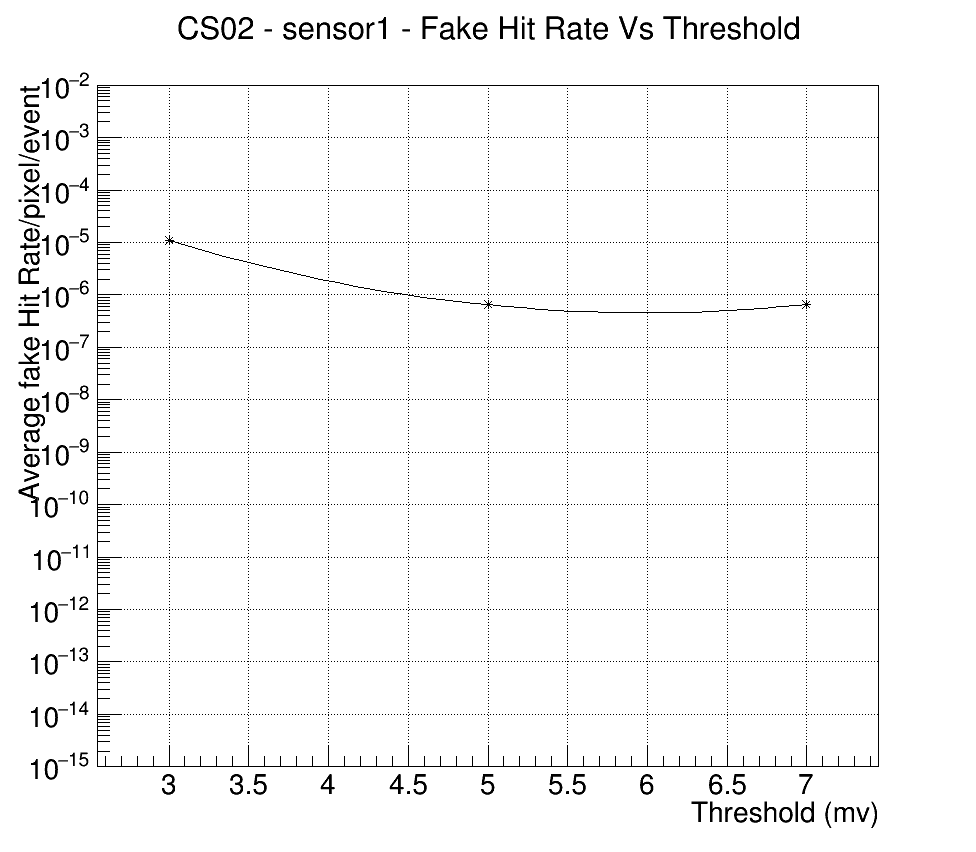
\includegraphics[width = 12cm]{Output_CS02_FHR/Fake_results_CS02_sensor1.png}
            \caption{Average Fake Hit Rate per pixel per event as a function of the Threshold.}
        \end{figure}
    \FloatBarrier 
        \begin{figure}[!h]
            \centering
            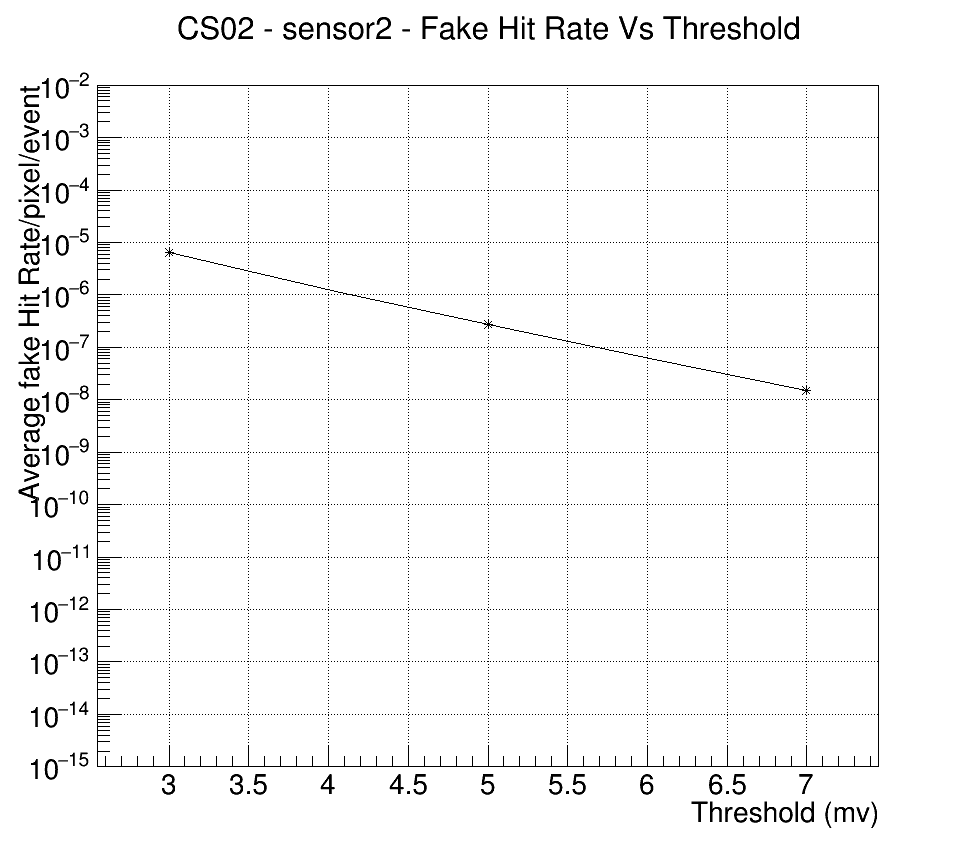
\includegraphics[width = 12cm]{Output_CS02_FHR/Fake_results_CS02_sensor2.png}
            \caption{Average Fake Hit Rate per pixel per event as a function of the Threshold.}
        \end{figure}
    \FloatBarrier 

  \begin{center}
    \begin{tabular}{|c|c|c|}
      \hline %----------------------------
   \rowcolor{light-gray}  Sensors  &  Run number  &  Thresholds  ($\sigma$) \tabularnewline
      \hline %----------------------------
      3-4   &   7081   &    3 \tabularnewline
      \hline %----------------------------
      3-4   &   7082   &    5 \tabularnewline
      \hline %----------------------------
      3-4   &   7083   &    7 \tabularnewline
      \hline %----------------------------
    \end{tabular}
  \end{center}

          \begin{figure}[!h]
            \centering
            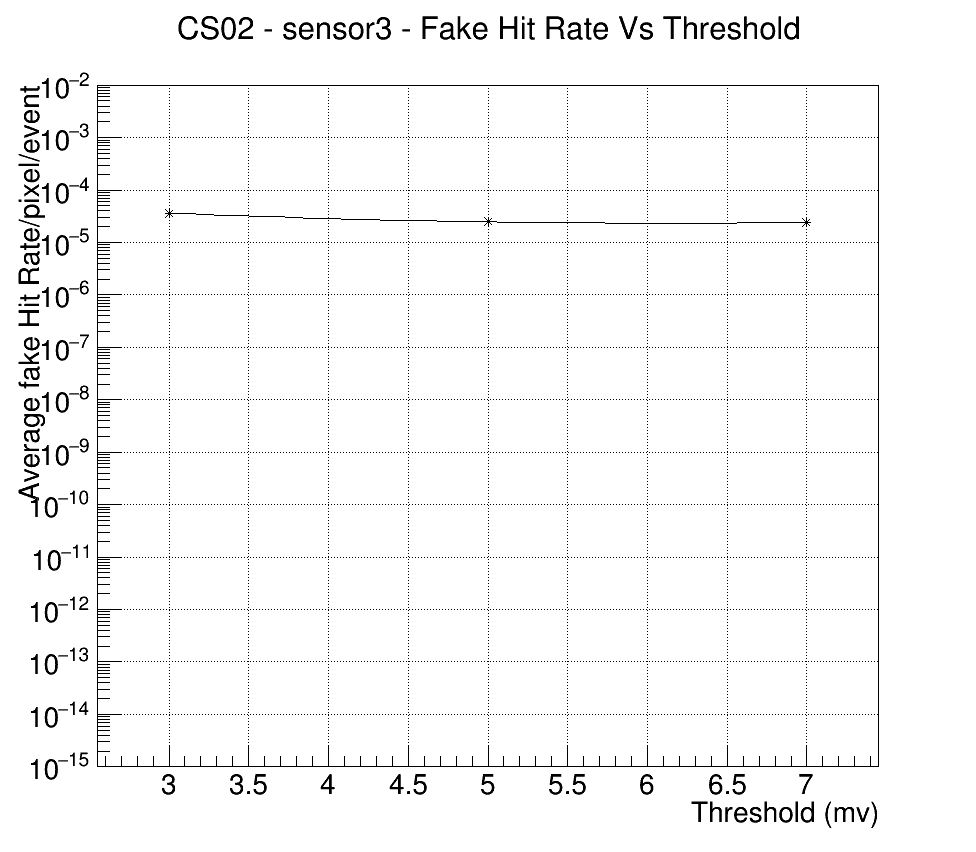
\includegraphics[width = 12cm]{Output_CS02_FHR/Fake_results_CS02_sensor3.png}
            \caption{Average Fake Hit Rate per pixel per event as a function of the Threshold.}
        \end{figure}
    \FloatBarrier 
        \begin{figure}[!h]
            \centering
            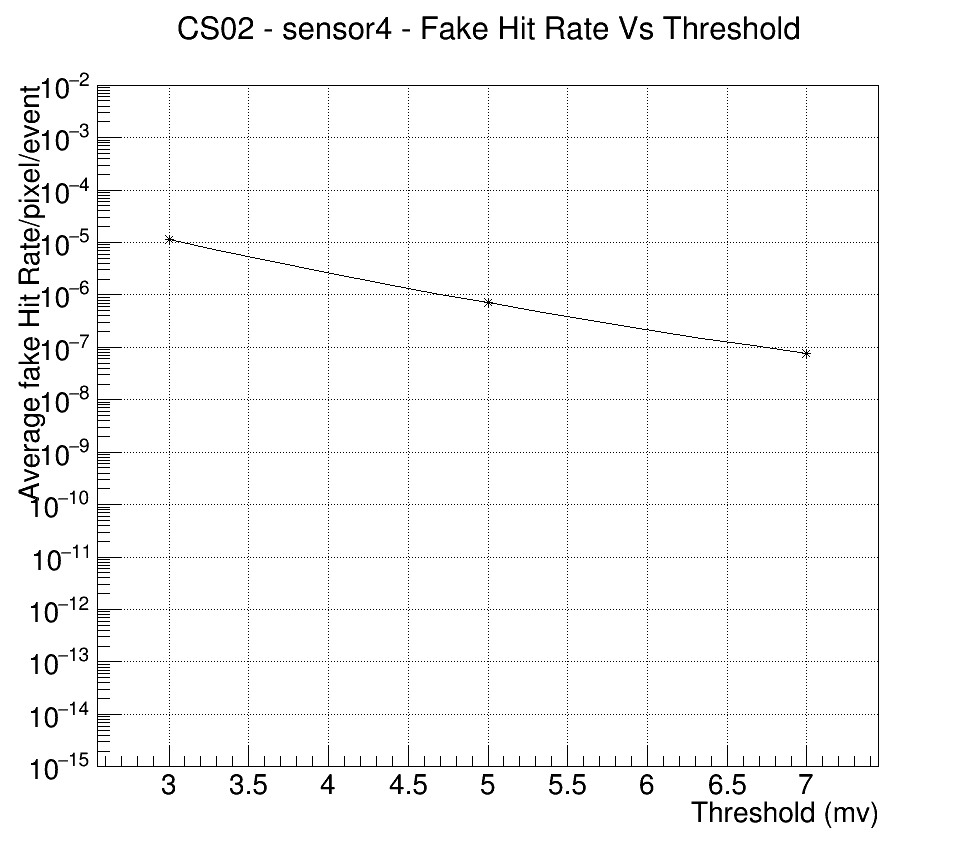
\includegraphics[width = 12cm]{Output_CS02_FHR/Fake_results_CS02_sensor4.png}
            \caption{Average Fake Hit Rate per pixel per event as a function of the Threshold.}
        \end{figure}
    \FloatBarrier 

  \begin{center}
    \begin{tabular}{|c|c|c|}
      \hline %----------------------------
   \rowcolor{light-gray}  Sensors  &  Run number  &  Thresholds  ($\sigma$) \tabularnewline
      \hline %----------------------------
      5-6   &   7084   &    3 \tabularnewline
      \hline %----------------------------
      5-6   &   7085   &    5 \tabularnewline
      \hline %----------------------------
      5-6   &   7086   &    7 \tabularnewline
      \hline %----------------------------
    \end{tabular}
  \end{center}

          \begin{figure}[!h]
            \centering
            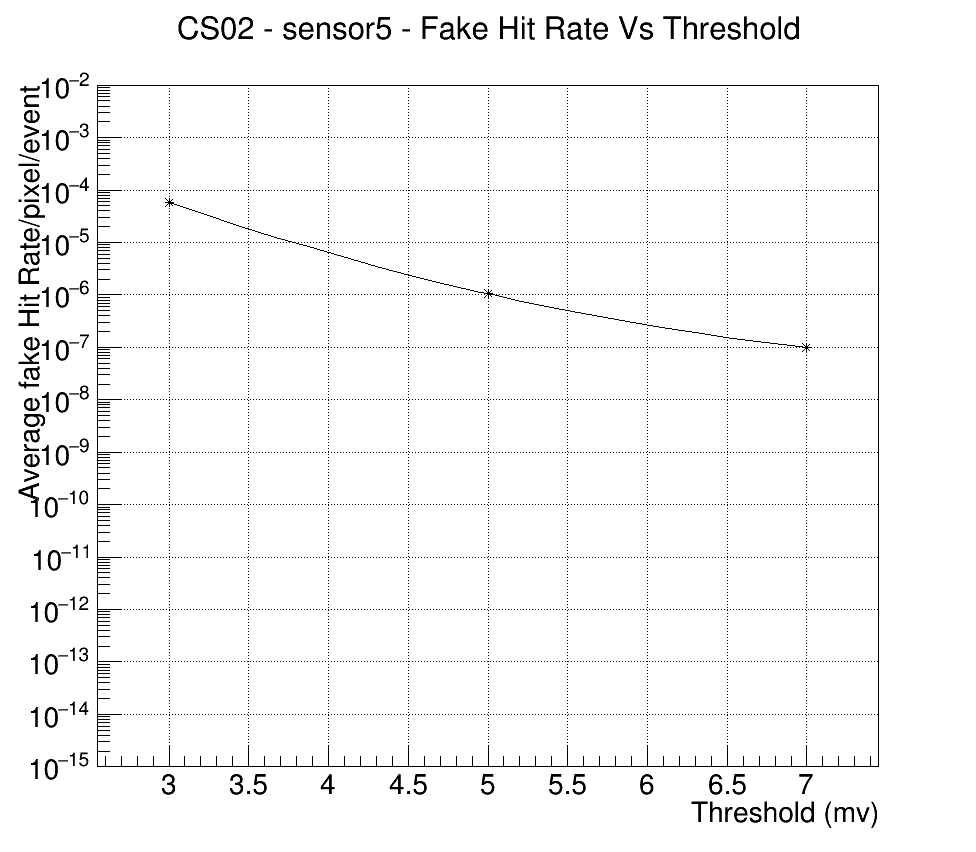
\includegraphics[width = 12cm]{Output_CS02_FHR/Fake_results_CS02_sensor5.png}
            \caption{Average Fake Hit Rate per pixel per event as a function of the Threshold.}
          \end{figure}
    \FloatBarrier 
        \begin{figure}[!h]
            \centering
            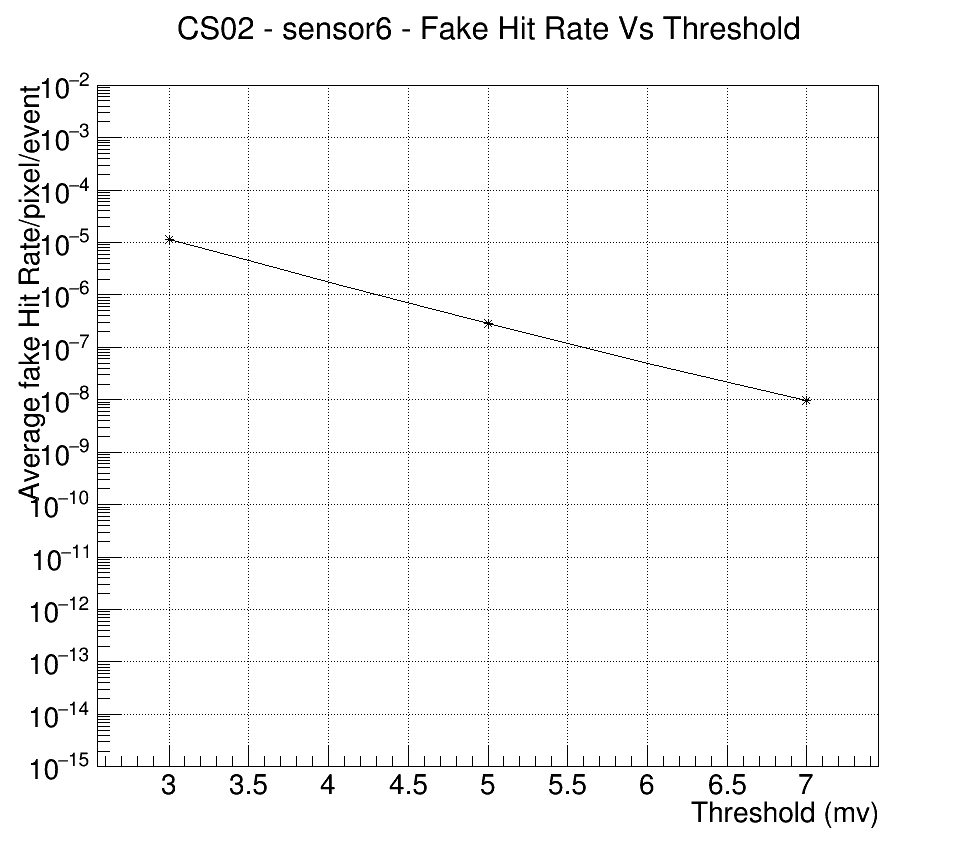
\includegraphics[width = 12cm]{Output_CS02_FHR/Fake_results_CS02_sensor6.png}
            \caption{Average Fake Hit Rate per pixel per event as a function of the Threshold.}
        \end{figure}
    \FloatBarrier 

 \end{document}
